\documentclass{article}
\usepackage{amsmath,bm,upgreek}
\usepackage{graphicx}
\usepackage{enumitem}
\usepackage{booktabs}
\usepackage{tcolorbox,newfloat}
\usepackage{tocloft}
\usepackage[hang,flushmargin]{footmisc}
\usepackage[margin=2cm]{geometry}
\usepackage[colorlinks,linkcolor=blue,citecolor=purple]{hyperref}
\usepackage[backend=bibtex,citestyle=numeric,
            maxcitenames=2,isbn=false,url=false]{biblatex}
% --------------------------------------------------------------------------------------------------
% paths
\graphicspath{{figs/}{figs/tikz/}}
\usepackage{tikz}
\usepackage{tikz-qtree}
\usetikzlibrary{positioning,arrows.meta,quotes,calc}
\tikzset{%
  arrow/.style    = { ->, >=Latex,  line width = 0.4mm, rounded corners, draw = black, every edge/.style={arrow} },
  arrow/.style    = { ->, >=Latex,  very thick, rounded corners,
                      fill = #1, draw = #1 },
  tbox/.style     = { fill = #1!20!white, draw = #1!80!white, thick, align = center,
                      minimum width = 0.8cm, minimum height = 0.6cm, node distance = 1.5cm },
  leaf/.style     = { fill = #1!20!white, draw = #1!80!white, thick, align = center, rounded corners = 0.3cm, grow = down,
                      minimum width = 1.2cm, minimum height = 0.6cm, node distance = 1.5cm }
}
\newcommand{\connectall}[2]{
  \foreach \s in {#1} {
    \foreach \t in {#2} {
      \draw[arrow,<->] (\s) -- (\t);
    }
  }
}
\bibliography{../../refs/refs.bib}
% formatting
\setlength{\cftbeforesecskip}{8pt}
\setlength{\parindent}{0pt}
\setlength{\parskip}{6pt}
\setlist[enumerate,1]{label=\arabic*.}
\setlist[enumerate,2]{label*=\arabic*.}
\numberwithin{equation}{section}
\newtcolorbox{fboxed}{sharp corners = all, colback = white!97!black, boxrule=1pt}
\DeclareFloatingEnvironment[name=Box]{floatbox}
\newcommand{\eq}[1]{Eq.~(\ref{#1})}
\renewcommand{\zeta}{\upzeta}
\newcommand{\x}{\hat{x}}
\newcommand{\e}{\hat{e}}
\newcommand{\N}{\textsc{n}}
\newcommand{\G}{\textsc{g}}
\newcommand{\citet}[1]{\citeauthor{#1}~(\citeyear{#1})~\cite{#1}}
% --------------------------------------------------------------------------------------------------
\title{Risk Group Dynamics in Simulated STI Epidemics}
\author{Jesse Knight}
%%%%%%%%%%%%%%%%%%%%%%%%%%%%%%%%%%%%%%%%%%%%%%%%%%%%%%%%%%%%%%%%%%%%%%%%%%%%%%%%%%%%%%%%%%%%%%%%%%%%
%%%%%%%%%%%%%%%%%%%%%%%%%%%%%%%%%%%%%%%%%%%%%%%%%%%%%%%%%%%%%%%%%%%%%%%%%%%%%%%%%%%%%%%%%%%%%%%%%%%%
%%%%%%%%%%%%%%%%%%%%%%%%%%%%%%%%%%%%%%%%%%%%%%%%%%%%%%%%%%%%%%%%%%%%%%%%%%%%%%%%%%%%%%%%%%%%%%%%%%%%
\begin{document}
%%%%%%%%%%%%%%%%%%%%%%%%%%%%%%%%%%%%%%%%%%%%%%%%%%%%%%%%%%%%%%%%%%%%%%%%%%%%%%%%%%%%%%%%%%%%%%%%%%%%
\maketitle
\tableofcontents
\subsection*{Key Contributions}
\begin{enumerate}
  \item Formalize a mathematical framework for risk group dynamics
  \item Describe methods for deriving risk group dynamics parameters from common data sources
  \item Illustrate differences in modelled projections for different implementations of risk group dynamics,
  using an example sexually transmitted infection
\end{enumerate}
\clearpage
%%%%%%%%%%%%%%%%%%%%%%%%%%%%%%%%%%%%%%%%%%%%%%%%%%%%%%%%%%%%%%%%%%%%%%%%%%%%%%%%%%%%%%%%%%%%%%%%%%%%
\section{Background}\label{s:background}
** R O U G H **
\begin{itemize}
  \item key factors in risk of HIV acquisition
  \item intro HIV modelling, prior work showing importance of heterogeneity
  \item comments on applicability of these concepts to non-HIV transmissible diseases
        (other STI, non-S TI)
  \item prior work on turnover, comment on need for ``equilibration'' / ``burn-in'' period
\end{itemize}
What do we mean by ``risk group dynamics''?
\begin{enumerate}
  \item inclusion of risk groups at all (yes / no)
  \item inclusion of turnover among these groups (yes / no, how?)
  \item consideration of how groups are re-balanced given differential attributable death
  -- subject of future work
\end{enumerate}
\par
From \citet{Eaton2014}:
\textit{Two behavioral parameters
-- the rate of transition from higher- to lower-risk groups and \textup{[\dots]} -- 
were particularly important for simulating the observed prevalence trend in many different ways,
as well as determining the intervention impact.}
\par
Some papers to include in Table~\ref{tab:prior-work-table}:
\cite{Barnighausen2012,Cremin2013,Eaton2014,Estill2012,Granich2009,Hallett2008,Johnson2006,Phillips2011,Rosenberg2004,Shah2016}
%%%%%%%%%%%%%%%%%%%%%%%%%%%%%%%%%%%%%%%%%%%%%%%%%%%%%%%%%%%%%%%%%%%%%%%%%%%%%%%%%%%%%%%%%%%%%%%%%%%%
\section{The System}\label{s:system}
This section introduces a system of compartments, flows, and equations
which can be used to describe risk group dynamics.
\par
We denote the variable representing
the size of risk group $i \in [1, \dots, \G]$ as $x_i$
and the vector of all $x_i$ as $\bm{x}$.
The total population size is denoted $\N = \sum_i x_i$,
and the proportions represented by each group by $\x_i = x_i \N^{-1}$.
The rate of population entry for all groups is denoted by $\nu$, and
the rate of exit by $\mu$.
We do not consider disease-attributable death, which may vary by group,
though this will be the subject of future work.
All rates have units \textit{per year} ($\mathrm{yr}^{-1}$).
The proportion of the entering population who are in group $i$,
which may not be equal to the proportion of the current population in group $i$,
is denoted $\e_i$.
Since the rate of entry $\nu$ is typically expressed as
a proportion of the total population size $\N$,
we model the theoretical entering population $\bm{e}$ as also having size $\N$,
so that $e_i = \e_i \N$.
\par
Turnover transitions can occur between any two groups, in either direction;
therefore we denote the turnover rates as a $\G \times \G$ matrix $\zeta$,
where $\zeta_{ij}$ corresponds to the transition $x_i \rightarrow x_j$.
An explicit definition is given in Eq.~(\ref{eq:zeta}),
where the diagonal elements are denoted $*$ since they represent
transitions from a group to itself, which is inconsequential.
\begin{equation}\label{eq:zeta}
\zeta = \left[\begin{array}{cccc}
         *           & x_1  \rightarrow x_2 & \cdots & x_1 \rightarrow x_\G \\[0.5em]
x_2  \rightarrow x_1 &          *           & \cdots & x_2 \rightarrow x_\G \\[0.5em]
      \vdots         &       \vdots         & \ddots &       \vdots         \\[0.5em]
x_\G \rightarrow x_1 & x_\G \rightarrow x_2 & \cdots &          *
\end{array}\right]
\end{equation}
These transition flows and the associated rates are summarized for $\G = 3$ in Figure~\ref{fig:system}.
\begin{figure}[h]
  \centering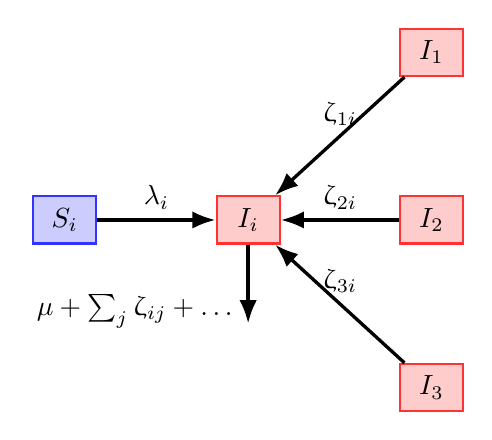
\begin{tikzpicture}
  \node(y)[tbox=red] {$I_i$};
  \node(s)[tbox=blue, left = of y]{$S_i$};
  \node(b)[tbox=red, right = of y]{$I_2$};
  \node(a)[tbox=red, above = of b]{$I_1$};
  \node(c)[tbox=red, below = of b]{$I_3$};
  \node(x)[below = of y]{};
  \draw[arrow,<-] (y) -- node[above] {$\lambda_{i}$} (s);
  \draw[arrow,<-] (y) -- node[above] {$\zeta_{1i}$} (a);
  \draw[arrow,<-] (y) -- node[above] {$\zeta_{2i}$} (b);
  \draw[arrow,<-] (y) -- node[above] {$\zeta_{3i}$} (c);
  \draw[arrow,->] (y) -- node[below left] {$\mu + \sum_j{\zeta_{ij}} + \dots$} (x);
\end{tikzpicture}
  \caption{System of compartments and flows between them for $\G = 3$}
  \label{fig:system}
\end{figure}
% ==================================================================================================
\subsection{Parameterization}
Next, we explore methods for estimating the values of parameters
in the system described above
($\nu$, $\mu$, $\bm{\x}$, $\bm{\e}$, and $\zeta$)
directly from some commonly available sources of data.
\par
In most cases, there will not be sufficient data to directly estimate all parameters,
especially $\zeta$.
The next section outlines additional methods to solve for these values.
\par
* (discuss latent assumptions with each of these approaches)

If we know the population size over time $\N(t)$, then \dots

If we know the annual growth rate over time $\mathcal{G}(t)$, then \dots

\begin{equation}\label{eq:pop-growth}
  \mathcal{G} = \nu - \mu
\end{equation}

If we know the duration of time spent in a particular group, then \dots

\begin{equation}\label{eq:duration}
  \mathcal{D}_i = {\left(\mu + \sum_{j}{\zeta_{ij}}\right)}^{-1}
\end{equation}

If we know the proportion $z$ of group $i$ who transition to group $j$ in a given year, then \dots

\begin{equation}
\zeta_{ij} = z
\end{equation}

Overall, we can write the system as a mass-balance equation,
so that the rate of change of group $x_i$
is simply the sum of flows in / out of the group,
\begin{equation}\label{eq:mass-balance}
  \frac{d}{dt}x_i
  = \nu \thinspace e_i + \sum_{j}{\zeta_{ji} \thinspace x_j}
  - \mu \thinspace x_i - \sum_{j}{\zeta_{ij} \thinspace x_i}
\end{equation}
While \eq{eq:mass-balance} is written in terms of absolute population sizes $\bm{x}$ and $\bm{e}$,
it is equivalent to divide through by $\N$, yielding a system in terms of $\bm{\x}$ and $\bm{\e}$,
the latter often proving more useful, since $\N$ need not be known.
% ==================================================================================================
\subsection{Solving the System}
In order to solve the system, we first note that the desired rate of change for risk group $i$
will be equal to the growth of the risk group, $\mathcal{G} x_i$.
Substituting this quantity into \eq{eq:mass-balance}, we have
\begin{equation}
  \mathcal{G}x_i = \nu \thinspace e_i + \sum_{j}{\zeta_{ji} \thinspace x_j}
                 - \mu \thinspace x_i - \sum_{j}{\zeta_{ij} \thinspace x_i}
\end{equation}
which, using the definition of $\mathcal{G}$ in \eq{eq:pop-growth}, we can simplify to
\begin{equation}
  \nu \thinspace x_i
      = \nu \thinspace e_i + \sum_{j}{\zeta_{ji} \thinspace x_j}
                           - \sum_{j}{\zeta_{ij} \thinspace x_i}
  \label{eq:system}
\end{equation}
% --------------------------------------------------------------------------------------------------
\subsubsection{Solving for $\zeta$}\label{sss:solve-zeta}
To solve for We rearrange \eq{eq:system} to obtain
\footnote{
  Using matrix notation, we \textit{could} rewrite the RHS of \eq{eq:system-zeta} as:
  ${({\bm{x}}^{\mathsf{T}}\zeta)}^{\mathsf{T}} - \zeta \thinspace \bm{x}$, % is this correct? cf. https://math.stackexchange.com/questions/2977829
  but this doesn't actually help us too much here.}
\begin{equation}\label{eq:system-zeta}
  \nu \left( x_i - e_i \right)
  = \sum_{j}{\zeta_{ji} \thinspace x_j}
  - \sum_{j}{\zeta_{ij} \thinspace x_i}
\end{equation}
which, considering all $i$, can be refactored to yield a system of the form:
\begin{equation}
\bm{b} = A \bm{z}
\end{equation}
where
$\bm{b} = \nu (\bm{x} - \bm{e})$ is a $\G$-length vector,
$A$ is a ${\G}\times\G^2$ matrix of coefficients, and
$\bm{z} = \mathrm{vec}(\zeta)$ is the $\G^2$-length vectorization of $\zeta$.
% --------------------------------------------------------------------------------------------------
\subsubsection{Solving for $e$}\label{sss:solve-e}
To solve for $\bm{e}$, we rearrange \eq{eq:system} to obtain
\begin{equation}\label{eq:system-e}
e_i = x_i - \left[ \sum_{j}{\zeta_{ji} \thinspace x_j}
                 - \sum_{j}{\zeta_{ij} \thinspace x_i} \right] \nu^{-1}
\end{equation}
% This final rearrangement is probably not useful, since we rarely know zeta, e, but not nu ...
%% --------------------------------------------------------------------------------------------------
%\subsubsection{Solving for $\nu$}
%To solve for $\nu$, we rearrange \eq{eq:system} to obtain
%\begin{equation}\label{eq:system-nu}
%  \nu = \left[ \sum_{j}{\zeta_{ji} \thinspace x_j}
%             - \sum_{j}{\zeta_{ij} \thinspace x_i} \right]
%       {\left( x_i - e_i \right)}^{-1}
%\end{equation}
%We actually cannot use this system to solve for $\mu$, however,
%because this term factors out of \eq{eq:system}.
% --------------------------------------------------------------------------------------------------
\subsubsection{Numerical Solutions}
* (from \texttt{/docs/idea/turnover.pdf}, \S~2.2)
\par
* This is only applicable to \ref{sss:solve-zeta}, should rearrange \dots
% ==================================================================================================
\subsection{Previous Approaches}
In this section, we will examine previous approaches to modelling
risk groups in simulated HIV epidemics,
and the assumptions inherent to these methods.
Box~\ref{box:assumptions} summarizes
the most common assumptions regarding the dynamics of these risk groups,
while Table~\ref{tab:prior-work-table} summarizes previous works
with respect to these assumptions.
\par
Many of the previously proposed models of HIV transmission
follow Assumption~\ref{ass:risk-groups-no} and do not consider heterogeneity
in risk of acquisition within major demographic groups,
such as heterosexual men / women, and MSM.
This is a significant assumption,
and may lead to large discrepancies with models which do consider risk heterogeneity,
as explored in Section~\ref{s:exp}.
Moreover, this assumption precludes any consideration of turnover,
since there is only one risk group, $\G = 1$.
\par
* (discussion of each assumption in turn)
\begin{floatbox}
  \caption{Common assumptions regarding the dynamics of risk groups}
  \label{box:assumptions}
  \begin{fboxed}
  \begin{enumerate}[leftmargin=1em]
    \item\label{ass:risk-groups}\textbf{Risk Groups:}
    Populations are stratified by risk of infection acquisition.
    \begin{enumerate}
      \item\label{ass:risk-groups-no}\textbf{No:} $G = 1$;
      Populations are homogeneous in risk of infection acquisition.
      \item\label{ass:risk-groups-yes}\textbf{Yes:} $G > 1$;
      Heterogeneity in risk of infection acquisition within populations is considered.
    \end{enumerate}
    \item\label{ass:turnover}\textbf{Turnover:}
    Individuals may move between risk groups.
    \begin{enumerate}
      \item\textbf{No:} $\zeta = 0$;
      Individuals do not move between risk groups.
      \item\textbf{Constant:} $\zeta > 0$;
      Individuals move between risk groups at a constant rate.
%      \item\textbf{Dynamic:} $\zeta = f$;
%      Individuals move between risk groups in dynamically.
    \end{enumerate}
    \item\label{ass:pop-growth}\textbf{Population Growth:}
    Increase in the total $N$ over time.
    \begin{enumerate}
      \item\textbf{No:} $\nu = \mu$;
      Population size $N$ is constant.
      \item\textbf{Yes:} $\nu > \mu$;
      Population size $N$ increases, at some constant or data-driven rate.
    \end{enumerate}
  \end{enumerate}
\end{fboxed}

\end{floatbox}
\begin{table}
  \centering
  \caption{Summary of prior work with respect to modelled risk group dynamics.}
  \label{tab:prior-work-table}
  \begin{tabular}{cllcccc}
	\toprule
	         Ref.           & Year                        & Author                        & Risk Groups $\G$ & Mortality $\phi$ & Dynamic Rebalance $RB$ & Turnover $\zeta$ \\
	\midrule
	  \cite{Hallett2008}    & \citeyear{Hallett2008}      & \citeauthor{Hallett2008}      &        3         &       Yes        &          None          &       None       \\
	\cite{Barnighausen2012} & \citeyear{Barnighausen2012} & \citeauthor{Barnighausen2012} &        1         &       Yes        &          None          &       N/A        \\
	   \cite{Estill2012}    & \citeyear{Estill2012}       & \citeauthor{Estill2012}       &        1         &       Yes        &          None          &       N/A        \\
	   \cite{Cremin2013}    & \citeyear{Cremin2013}       & \citeauthor{Cremin2013}       &        3         &       Yes        &          None          &       None       \\
	   \cite{Eaton2014}     & \citeyear{Eaton2014}        & \citeauthor{Eaton2014}        &        3         &       Yes        &          None          &     Constant     \\
	                        &                             & \dots \\
	\bottomrule            
\end{tabular}

\end{table}
\clearpage
%%%%%%%%%%%%%%%%%%%%%%%%%%%%%%%%%%%%%%%%%%%%%%%%%%%%%%%%%%%%%%%%%%%%%%%%%%%%%%%%%%%%%%%%%%%%%%%%%%%%
\section{Experiment}\label{s:exp}
Next, we will explore differences in projected model outputs
under different implementations of risk groups dynamics,
using a simple model of heterosexual HIV transmission.
% ==================================================================================================
\subsection{Model Overview}
Our model of HIV transmission includes 3 health states (Figure~\ref{fig:health-states}),
and 3 levels of sexual activity (risk groups, $\G = 3$).
\dots
\begin{table}
  \centering\caption{Model parameters -- e.g. table}
  \label{tab:model-params}
  \begin{tabular}{clcc}
  	\toprule
  	Symbol  & Description                                 & Value & Sampled Range \\
  	\midrule
  	$\beta$ & Probability of transmission per partnership & e.g.  & e.g. \\
  	        & \dots                                       &       & \\
  	\bottomrule
  \end{tabular}
\end{table}

\begin{figure}
  \centering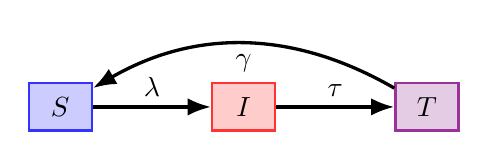
\begin{tikzpicture}
\node(S) [tbox=blue] at (0.0,0.0)   {$S$};
\node(I) [tbox=red,    right = of S]{$I$};
\node(T) [tbox=violet, right = of I]{$T$};

\draw[arrow=black] (S) edge["$\lambda$"] (I);
\draw[arrow=black] (I) edge["$\tau$"]  (T);
\draw[arrow=black] (T) edge["$\gamma$", bend right] (S);
\end{tikzpicture}
  \caption{Modelled health states}\label{fig:health-states}
\end{figure}
% ==================================================================================================
\subsection{Model Variants}\label{ss:model-variants}
Drawing on the most common assumptions outlined in Box~\ref{box:assumptions},
we define a series of model variants for investigation;
these variants are summarized in Figure~\ref{fig:variant-tree}.
\begin{figure}
  \centering\newlength{\lvl}\setlength{\lvl}{1.2cm}
%\begin{tikzpicture}[
%    level distance = \lvl,
%    edge from parent/.append style = { draw = none } 
%  ]
%  \Tree [.{} [.{$\G$} [.{$\zeta$} ] ] ] 
%\end{tikzpicture}\hspace{0.5\lvl}
\begin{tikzpicture}[
    level distance = \lvl,
    sibling distance = 0.4\lvl,
    every path/.append style = { thick },
    edge from parent path = {
      (\tikzparentnode) -- +(0.0,-0.5\lvl) -| (\tikzchildnode)
    }
  ]
  \Tree
    [.{}
      [.\node[leaf=gray]{$\G=1$};
        [.\node[leaf=gray]{$\cdot$}; ]
      ]
      [.\node[leaf=gray]{$\G=3$};
        [.\node[leaf=gray]{$\zeta = 0$}; ]
        [.\node[leaf=gray]{$\zeta = C$}; ]
      ]
    ]
\end{tikzpicture}

  \caption{Summary of 3 model variants with respect to models of population turnover.
    $\G$:~number of risk groups,
    $\zeta$:~rates of population turnover,
    $(\thinspace\cdot\thinspace)$:~not applicable,
    $C$:~a constant}
  \label{fig:variant-tree}
\end{figure}
% ==================================================================================================
\subsection{Simulations}
The simulated epidemic is initialized in 1975 with \dots

* Describe the scenario
\par
This epidemic was simulated
using each of the model variants described in \S~\ref{ss:model-variants}.
In each case, we compared the model predictions across the variants
regarding three outputs:
\begin{enumerate}
  \item Projected prevalence for $t = 1975 - 2050$
  \item Population attributable fraction of highest risk group (variants with $\G = 3$ only)
  \item Estimated impact of \{intervention x -- ART?\} at reducing cumulative new infections between 2020 and 2050
\end{enumerate}
\dots
\par
Since the results of these comparisons are significantly affected by several model parameters,
we performed a comprehensive sensitivity analysis.
The parameter ranges specified in Table~\ref{tab:model-params} were used,
and \dots

* (construct a GLM or something to describe the impacts?)
%%%%%%%%%%%%%%%%%%%%%%%%%%%%%%%%%%%%%%%%%%%%%%%%%%%%%%%%%%%%%%%%%%%%%%%%%%%%%%%%%%%%%%%%%%%%%%%%%%%%
\section{Results}\label{s:results}

\begin{figure}
  \centering\scalebox{6}{$\times$}
  \caption{Projected prevalence under each of the 10 model variants.}
\end{figure}
\begin{figure}
  \centering\scalebox{6}{$\times$}
  \caption{Estimated impact of \{intervention x\} on cumulative new infections between 2020 and 2050.}
\end{figure}
%%%%%%%%%%%%%%%%%%%%%%%%%%%%%%%%%%%%%%%%%%%%%%%%%%%%%%%%%%%%%%%%%%%%%%%%%%%%%%%%%%%%%%%%%%%%%%%%%%%%
\section{Discussion}\label{s:discussion}
%%%%%%%%%%%%%%%%%%%%%%%%%%%%%%%%%%%%%%%%%%%%%%%%%%%%%%%%%%%%%%%%%%%%%%%%%%%%%%%%%%%%%%%%%%%%%%%%%%%%
\section{Conclusions}\label{s:conclusion}
%%%%%%%%%%%%%%%%%%%%%%%%%%%%%%%%%%%%%%%%%%%%%%%%%%%%%%%%%%%%%%%%%%%%%%%%%%%%%%%%%%%%%%%%%%%%%%%%%%%%
\section{References}\label{s:references}
\printbibliography[heading=none]
%%%%%%%%%%%%%%%%%%%%%%%%%%%%%%%%%%%%%%%%%%%%%%%%%%%%%%%%%%%%%%%%%%%%%%%%%%%%%%%%%%%%%%%%%%%%%%%%%%%%
\end{document}
%%%%%%%%%%%%%%%%%%%%%%%%%%%%%%%%%%%%%%%%%%%%%%%%%%%%%%%%%%%%%%%%%%%%%%%%%%%%%%%%%%%%%%%%%%%%%%%%%%%%
%%%%%%%%%%%%%%%%%%%%%%%%%%%%%%%%%%%%%%%%%%%%%%%%%%%%%%%%%%%%%%%%%%%%%%%%%%%%%%%%%%%%%%%%%%%%%%%%%%%%
%%%%%%%%%%%%%%%%%%%%%%%%%%%%%%%%%%%%%%%%%%%%%%%%%%%%%%%%%%%%%%%%%%%%%%%%%%%%%%%%%%%%%%%%%%%%%%%%%%%%